\documentclass{article}
\usepackage{listings}
\usepackage{pdfpages}
\graphicspath{ {.} }

\usepackage{fancyhdr}
\usepackage[pdftex,
    pdfauthor={Aryan Gupta},
    pdftitle={ECGR4181 HW4 Report},
    pdfsubject={Homework Report},
    pdfkeywords={},
    pdfproducer={Latex with hyperref},
    pdfcreator={}
]{hyperref}
\usepackage[margin=1in]{geometry}
\hypersetup{colorlinks=true, linkcolor=black,urlcolor=black}
\usepackage[margin=1in]{geometry}
\usepackage{lastpage}
\usepackage[margin=1in]{geometry}
\usepackage{fancyhdr}
\usepackage{amsmath,amsfonts, amsthm}
\usepackage{float}
\usepackage{graphicx}
\usepackage{courier}

\lstset{
    basicstyle=\ttfamily,
    frame=single,
}

\begin{document}
    \section{Code}
    The code written for this assignment comprised of many parts, however much of the code was borrowed from the previous homework’s. All the code is contained in the \texttt{src/} directory. The first two classes I would like to talk about are the \texttt{BitCounter} and the \texttt{ShiftRegister}. These are two classes that assist in the running of various of the branch predictors. The \texttt{BitCounter} class is a class that implements a bit counter. The high value (max) value can be defined during compile time using template parameters. I added a feature that depending on how many bits you need the \texttt{BitCounter} or \texttt{ShiftRegister}, the underlying int type will automatically be chosen to the smallest int that can fit the requirements. For example, if we wanted to create a 10bit shift register, then we would create the class using \texttt{ShiftRegister<10>}. The program will automatically choose \texttt{uint16\_t} to be the underlying type because it has at least 10 bits. Another example is if we need a 2 bit shift register then declaring \texttt{ShiftRegister<2>} will pick \texttt{uint8\_t} as the underlying type because it has enough bits to store out 2 bit value. \par
    The classes use bit masking and other bit manipulation techniques to keep their invariants. Both classes are \texttt{constexpr} class so it is all defined in the header. The \texttt{Simulator} class idea was taken from Homework 1, and is the class that runs the actual simulations. The simulator first calls the branch predictor and requests a guess. If the guess is correct it adds 1 to the correct count. It also keeps a count of total number of branches. Then it calls the branch predictor again with the correct value and the guess that it gave so the branch predictor can take measures to improve its accuracy. The parse file was also taken from Homework 1 and slightly modified to suit the needs of this homework. \par
        \subsection{Branch Predictors}
        Because there was a number of branch predictors that were created, I added them to its own \texttt{namespace} called \texttt{BranchPredictorTypes}. The various branch predictors are implemented as a derived class of an interface called \texttt{BranchPredictor}. The interface only contains two functions.
        \begin{lstlisting}[language=C++]
virtual bool operator()(addr_t a) = 0;
virtual void operator()(addr_t a, bool b, bool c) = 0;
        \end{lstlisting}
        The first function passes in an argument \texttt{a}, which is the address the simulator would like a guess for. The function returns true if the branch should be taken (this is the branch predictor's guess) and false if it should not be taken. The second function is called by the simulator so the branch predictor can update its internal state depending on whether the branch was actually taken or not. \texttt{b} is the actual result of the branch, and \texttt{c} is the guess that the branch predictor predicted from function one. The abstract class also has a function:
        \begin{lstlisting}[language=C++]
template <std::size_t B = 10>
static constexpr addr_t get_sbits(addr_t addr)
        \end{lstlisting}
        This function simply returns the last \texttt{B} bits of the address \par
        Each branch predictor is a child class of this interface. For example, the branch predictor \texttt{Always} always takes a branch or doesn't take a branch depending on its c'tor call.
        \begin{lstlisting}[language=C++]
Always::Always(bool taken) : mTaken{ taken } {}

bool Always::operator()(addr_t addr) {
    return mTaken;
}

void Always::operator()(addr_t addr, bool taken, bool guess) {
    return;
}
        \end{lstlisting}
        In this code snippet, it can be seen that if the \texttt{Always} branch predictor is initialized with true (\texttt{Always\{ true \}}) then the branch predictor will always take the branch; however if the branch predictor is initialized with false then the branch predictor will never take the branch. \par
        A more concrete example can be seen with the \texttt{TwoBit} branch predictor.
        \begin{lstlisting}[language=C++]
class TwoBit {
    using counter_t = BitCounter<2>;
    std::array<counter_t, 1024> mPHT;
// Excluded for brevity. See TwoBit.hpp for complete listing
};

bool TwoBit::operator()(addr_t addr) {
    addr_t idx = get_sbits(addr);
    return mPHT[idx].value() >= (counter_t::max() / 2);
}

void TwoBit::operator()(addr_t addr, bool taken, bool) {
    if (taken) {
        ++mPHT[get_sbits(addr)];
    } else {
        --mPHT[get_sbits(addr)];
    }
}
        \end{lstlisting}
        In this code listing, it can be seen that our \texttt{TwoBit} branch predictor has one member variable called \texttt{mPHT} that is an array of our 2-bit counter. The branch predictor looks up the address of the branch instruction (\texttt{operator()(addr\_t)}) and then tests if that bit counter is more than half of the max value. In case of our 2 bit bit counter each state is represented by \texttt{\{ 0 : Strongly Not Taken, 1 : Not Taken, 2 : T, 3 : ST \}}. By comparing the value with \texttt{max() / 2}, it allows us to change the bit counter size in part 2 of this homework. Then after the simulator recives the guess. The simulator runs the other operator: \texttt{operator()(addr\_t, bool, bool)}, this operator updates our internal state depending on the actual outcome of the branch. For the two bit branch predictor, if the branch was taken then the corresponding counter is incremented. Remember that we defied our bit counter such that the value cannot exceed the max value. For our 2 bit counter here, the max value is 4 so the value cannot exceed 3, similar for the low end (value: 0). \par
        The other branch predictors are implemented in a similar fashion. Where the derived class has member variables holding the state of the branch predictors and there are 2 function that work on the data to produce an prediction for the branch. It would be helpful if the trace had where the branch jumped to, this way we could implement a backwards-always-taken-forward-not-taken branch predictor. The complete list of branch predictors and their command line arguments are listed below:
        \begin{itemize}
            \item Always Taken          -pAlwaysT
            \item Always Not Taken      -pAlwaysN
            \item One Bit               -pOneBit
            \item Two Bit               -pTwoBit
            \item Two Level Global      -pGlobal
            \item Two Level GShare      -pGShare
            \item Two Level GSelect     -pGSelect
            \item Two Level Local       -pLocal
            \item Custom                -pCustom
        \end{itemize}
        The program can be simply run as:
        \begin{lstlisting}
            bin/main.out --file project/branch-trace-gcc.trace -pGSelect
        \end{lstlisting}
    \section{Results}
        The results in this homework was very interesting. I predicted that the GShare branch predictor or the Local branch predictor would perform the best however, this was not the case.
        \begin{figure}[H]
            \centering
            \label{fig:bp_results}
            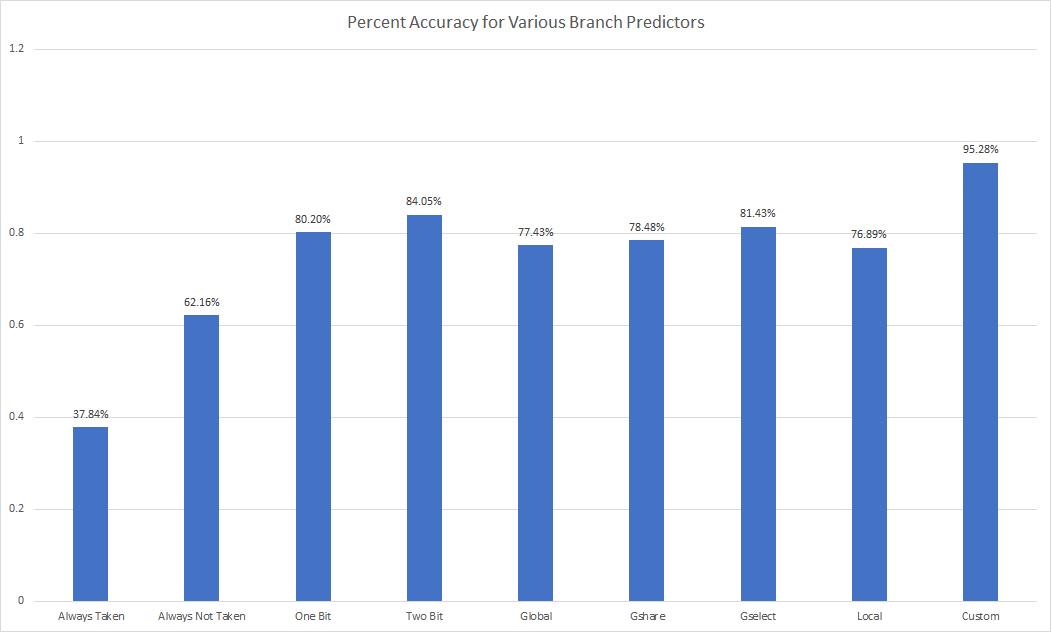
\includegraphics[width=\textwidth]{bp_results.png}
            \caption{Accuracy of various branch predictors}
        \end{figure}
        In Figure \ref{fig:bp_results}, it can be seen that the trace given to us challenged the branch predictor. I was unable to get the proper results. As you can see, the two bit branch predictor all of the other predictors. Out of the two level branch predictors, the local branch predictor performed the worst, when it should have been the best. \par
        When changing the saturation bit counter width, an interesting thing happened. The prediction rate went up but then sharply dropped.
        \begin{figure}[H]
            \centering
            \label{fig:sat_results}
            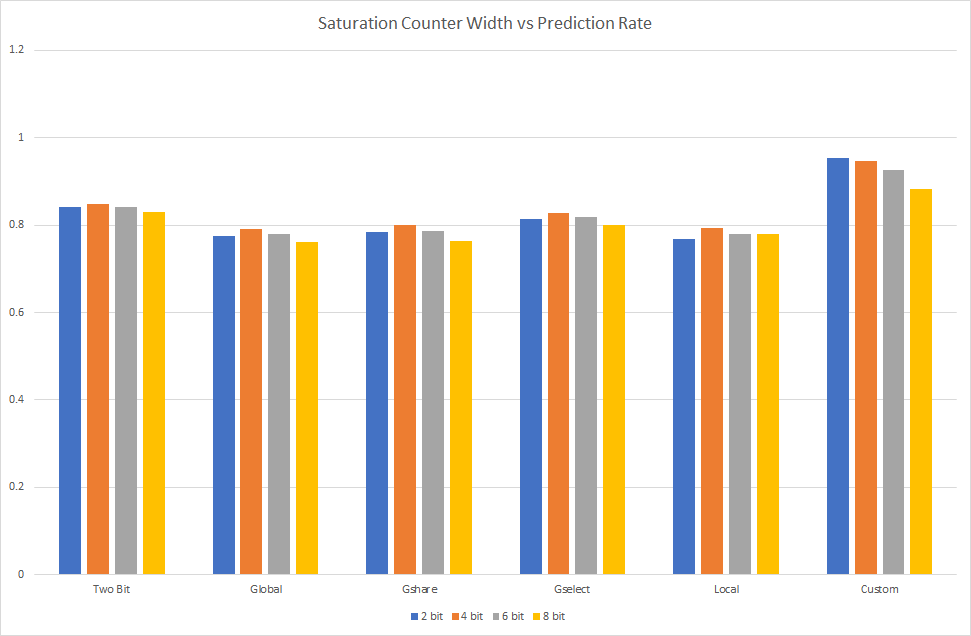
\includegraphics[width=\textwidth]{sat_results.png}
            \caption{Saturation Counter Width vs Prediction Rate}
        \end{figure}
        As shown in the graph, if the saturation bit counter is raised from 2 to 4 bits (note that this is in powers of 2 so in reality the counter was raised from 4 to 8), the prediction rate increases immensely, however any raise after that leads to diminishing returns and the prediction rate drops. The best bit width for the branch predictors seem to be 4 bit counter (from 0 to 8). This result can be seen across the board with all the predictors using the saturated counters.

    \section{Pintools}
        I was unable to get pintools working for branch prediction in time for the submission of this homework. I was constantly met with `A fatal error has occurred'.

    \section{Custom Branch Predictor}
        This may be very cliché and informal, however, this idea legit came to me in a dream. I was thinking, what if we keep a record of all the occurrences of a branch pattern (like the Global History Table does), for every local branch address (like the Local branch predictor does), and we use the global history table to reference it? I was so excited to try it out when I woke up and behold I got a 95\%. I was very excited about it and started playing around with various values to see if I could tweak it to get more performance, however I was unable to gain performance short of increasing the amount of branch predictor buffer we had. The performance can be seen in the Figure \ref{fig:bp_results} and Figure \ref{fig:sat_results}. The code can be found in \texttt{src/Custom.cpp}.
\end{document}

